\chapter{Tecnologie utilizzate}
\label{cha:tecnologieutilizzate}
In questa sezione vengono presentate, con un adeguato livello di dettaglio, le tecnologie utilizzate per la realizzazione della pipeline dati sviluppata durante il tirocinio. Lo stack tecnologico adottato è stato progettato per garantire modularità, scalabilità e osservabilità del sistema, caratteristiche fondamentali in un contesto di automazione e monitoraggio di processi dati periodici. Come si può notare, tutte le tecnologie utilizzate seguono la filosofia open source. Con il termine open source si intende software il cui codice sorgente è pubblico e liberamente accessibile: questo permette a chiunque di utilizzarlo, modificarlo e distribuirlo. Grazie a questa apertura, la collaborazione tra sviluppatori è facilitata e diventa più semplice correggere errori o aggiungere nuove funzionalità.


Le tecnologie possono essere suddivise in tre principali categorie funzionali:

\begin{itemize}
    \item \textbf{Containerizzazione}: Docker e Docker Compose sono stati utilizzati per creare un ambiente di esecuzione isolato, facilmente replicabile e portabile. Tutti i componenti dell'infrastruttura vengono eseguiti come container indipendenti ma coordinati, permettendo una gestione semplificata dell'intero sistema.
    \item \textbf{Orchestrazione}: Apache Airflow è stato scelto come strumento per l'automazione e la schedulazione dei flussi di lavoro. La sua interfaccia intuitiva e il paradigma configuration as code lo rendono adatto a definire e monitorare pipeline complesse.
    \item \textbf{Monitoraggio e raccolta delle metriche}: il sistema di osservabilità è stato implementato utilizzando StatsD Exporter, Prometheus e Grafana. Le metriche prodotte da Airflow vengono raccolte, elaborate e visualizzate in tempo reale tramite dashboard interattive, al fine di garantire il corretto funzionamento del sistema e facilitare l'identificazione di anomalie o colli di bottiglia.
\end{itemize}

Nei paragrafi seguenti, ogni tecnologia verrà descritta singolarmente.



\section{Docker}
\label{sec:docker}
Docker è una piattaforma open-source che consente di creare, distribuire ed eseguire applicazioni all'interno di pacchetti detti container. È importante notare che quando si parla di Docker, di solito ci si riferisce a Docker Engine, il software che ospita i container. Docker utilizza la virtualizzazione a livello di sistema operativo (containerizzazione), in particolare utilizza alcune feature del Kernel Linux per garantire l’isolamento e il controllo dei pacchetti. Alcuni esempi di strumenti del Kernel che vengono utilizzati sono i cgroup e i namespace. I cgroups (control groups) sono una funzionalità del kernel linux che permette di limitare, monitorare e assegnare le risorse del sistema ai diversi processi in esecuzione. In questo modo, ogni container può essere configurato per utilizzare solo una certa quantità di risorse, evitando che un singolo container possa consumare tutte le risorse dell’host a discapito degli altri.
I namespace, invece, sono un meccanismo che isola la visione che ha un’applicazione delle risorse di sistema. Grazie ai namespace, ogni container vede solo i processi, le interfacce di rete, i punti di mount e le variabili d’ambiente che gli sono stati assegnati, come se fosse l'unico sistema attivo sulla macchina. Questo garantisce un elevato livello di isolamento rispetto agli altri container e al sistema operativo. Questo approccio, basato sulla containerizzazione \ref{fig:docker_containerization}, rende i container molto più leggeri (nell’ordine di megabyte, contro i gigabyte di molte VM)[IBM docker] e più rapidi da avviare rispetto alle macchine virtuali tradizionali. L’efficienza ottenuta consente di eseguire molti più container sullo stesso hardware rispetto alle VM e di rendere lo sviluppo e il deployment delle applicazioni più agili e flessibili.

\begin{figure}[h]
    \centering
    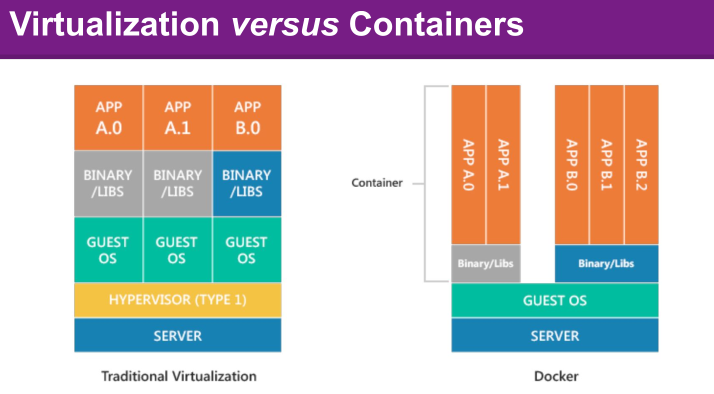
\includegraphics[width=0.8\textwidth]{img/contvsvirt.png}
    \caption{Confronto tra le macchine virtuali tradizionali e i container di Docker}
    \label{fig:docker_containerization}
\end{figure}

\subsection{Principali componenti}
\label{sec:principalicomponenti}

L’ecosistema Docker è composto da tre elementi principali:


\begin{itemize}
    \item \textbf{Software}: Il cuore del sistema è il Docker daemon (dockerd), un processo che gestisce i container e le altre risorse Docker. Gli utenti interagiscono con il daemon tramite il Docker Client, ovvero un'interfaccia a riga di comando (docker) che comunica attraverso le API di Docker Engine.
    \item \textbf{Oggetti}: Gli oggetti Docker rappresentano le entità fondamentali per il funzionamento delle applicazioni containerizzate. I principali sono:
    \begin{itemize}
        \item \textbf{Immagini}: template di sola lettura da cui vengono creati i container.
        \item \textbf{Container}: ambienti isolati in cui vengono eseguite le applicazioni.
        \item \textbf{Servizi}: permettono ai container di essere scalati su più Docker daemon creando così uno swarm (un insieme di di daemon cooperante tramite l'API di Docker).
    \end{itemize}
    Gli oggetti di Docker verranno trattati con maggiore dettaglio nelle seguenti sottosezioni.
    \item \textbf{Registry}: I registry sono archivi centralizzati dove vengono conservate le immagini Docker. Possono essere pubblici o privati; il più noto è Docker Hub, il registry predefinito. I registry permettono di caricare e scaricare immagini.
\end{itemize}


\subsection{Immagini e Dockerfile}
\label{sec:immaginiedockerfile}
Le applicazioni containerizzate in Docker vengono distribuite sotto forma di immagini Docker, ovvero template immutabili da cui si generano i container. Ogni immagine racchiude il file system e tutte le istruzioni necessarie per avviare l’applicazione all’interno di un container. La creazione di un’immagine è automatizzata tramite un file di configurazione testuale chiamato Dockerfile, in cui vengono specificati in modo dichiarativo tutti i passaggi necessari: dalla scelta dell’immagine di base (ad esempio una distribuzione Linux minimale), alla copia dei file dell’applicazione, fino all’installazione delle dipendenze e alla configurazione dell’ambiente (cartella di lavoro, utenti, variabili d’ambiente, ecc.). Questo approccio garantisce la riproducibilità e la coerenza dell’ambiente software, eliminando i tipici problemi di compatibilità tra sistemi diversi. Le immagini Docker possono inoltre essere versionate e facilmente condivise tramite i registry, favorendo la collaborazione e la distribuzione delle applicazioni.

\subsection{Container}
\label{sec:container}
Un container Docker è un’istanza attiva di un’immagine: rappresenta un ambiente isolato, leggero e portatile che esegue un’applicazione con tutte le sue dipendenze, come definito nell’immagine da cui è stato creato. Tuttavia, nella pratica, molte applicazioni moderne richiedono l’interazione tra più servizi distinti, ciascuno eseguito in un proprio container. Per gestire e orchestrare in modo semplice insiemi di container che compongono un’applicazione complessa si utilizza Docker Compose, uno strumento che permette di definire e avviare configurazioni multi-container tramite un unico file YAML.
Inoltre, poiché i container sono per loro natura effimeri e i dati scritti al loro interno vengono persi alla loro rimozione, Docker mette a disposizione i volumi: uno strumento pensato per garantire la persistenza dei dati e la condivisione delle informazioni tra container diversi o tra host e container.

\subsection{Docker Compose}
\label{sec:dockercompose}
Docker Compose è uno strumento che permette di definire, configurare e gestire applicazioni composte da più container. Tramite un file in formato YAML (docker-compose.yml), è possibile descrivere tutti i servizi che compongono l’applicazione, specificando per ciascuno l’immagine da usare, le variabili d’ambiente, le reti, le dipendenze e i volumi associati. Questo approccio consente di avviare, arrestare o aggiornare l’intero stack applicativo con un singolo comando, semplificando la gestione di architetture complesse e migliorando la riproducibilità degli ambienti sia in fase di sviluppo che di produzione. Compose è particolarmente utile quando si desidera far lavorare insieme più servizi (ad esempio un database, un’applicazione backend e un frontend), ciascuno eseguito nel proprio container ma coordinati tra loro.

\subsection{Volumi}
\label{sec:volumi}
I volumi in Docker rappresentano una soluzione per la persistenza dei dati nei container. Di default, i dati creati all’interno di un container sono temporanei e vengono eliminati quando il container viene rimosso. I volumi permettono di salvare dati in uno spazio dedicato e indipendente dal ciclo di vita dei singoli container, garantendo che le informazioni rimangano disponibili anche dopo la terminazione o la ricreazione dei container. Inoltre, i volumi possono essere utilizzati per condividere dati tra più container o per facilitare l’integrazione con il sistema host. Questa caratteristica è fondamentale per applicazioni che richiedono la conservazione dei dati, come database, sistemi di caching o storage di file.

Esistono due tipi di volumi:
\begin{itemize}
    \item \textbf{Bind Mount}: Consente di collegare una cartella o un file presente sul filesystem dell’host direttamente all’interno di uno o più container. Questo tipo di volume risulta particolarmente utile quando è necessario accedere a file specifici già esistenti o quando si dispone di spazio limitato sul disco gestito da Docker, poiché i dati vengono memorizzati direttamente nel percorso scelto sull’host.
    \item \textbf{Named Volume}: Si tratta di volumi gestiti direttamente da Docker, che vengono creati e organizzati in modo automatico dal Docker Engine all’interno di uno spazio dedicato dell’host. Sono ideali per la persistenza dei dati tra diverse esecuzioni dei container, e permettono una gestione più semplice e indipendente dal percorso fisico sul filesystem.
\end{itemize}

In generale, i bind mount sono consigliati quando si vuole controllare esattamente dove vengono salvati i dati o quando si ha poco spazio disponibile nell’area gestita da Docker, mentre i named volume offrono maggiore astrazione e portabilità nell’uso dei dati tra container diversi.




\section{Apache Airflow}
\label{sec:airflow}
Airflow è una piattaforma open-source progettata per la gestione automatizzata dei flussi di lavoro. Consente di definire, pianificare e monitorare in modo programmatico i workflow, tramite una pratica interfaccia utente integrata.
Creato originariamente da Airbnb, Airflow è sviluppato in Python ed è progettato secondo il paradigma del Configuration as Code. 

La Configuration-as-Code (CaC) è un approccio che prevede la gestione delle configurazioni tramite codice, invece che attraverso modifiche manuali o strumenti proprietari. In pratica, le configurazioni vengono trattate come vero e proprio codice applicativo. Questo metodo offre diversi vantaggi: garantisce coerenza e ripetibilità nelle configurazioni, riduce il rischio di errori umani e semplifica il ripristino in caso di problemi. Inoltre, essendo gestite come codice, le configurazioni possono essere versionate tramite sistemi di controllo versione (come Git), permettendo di tracciare facilmente le modifiche e tornare a versioni precedenti se necessario.

Airflow sfrutta Python per definire i flussi, a differenza di altre piattaforme simili, che tipicamente utilizzano linguaggi markup come XML. Questo approccio permette agli sviluppatori di importare librerie o script esistenti nel loro workflow.

Ogni workflow viene rappresentato come un DAG (Directed Acyclic Graph), ovvero un grafo orientato e aciclico, dove i nodi rappresentano i task (le singole operazioni da eseguire) e le frecce rappresentano le dipendenze e l’ordine di esecuzione tra i task.


\subsection{Concetti principali}
\label{sec:concettiprincipali}
Per comprendere il funzionamento di Apache Airflow, è fondamentale introdurre alcuni concetti chiave che costituiscono la base della piattaforma e ne determinano la logica operativa.

Tra questi i principali sono:
\begin{itemize}
    \item \textbf{DAG}: è la struttura fondamentale che descrive un workflow, ossia una sequenza di operazioni da eseguire secondo una precisa logica di dipendenze.
    Un DAG definisce quali task devono essere eseguiti e in quale ordine, rappresentando graficamente e logicamente il flusso di lavoro in cui ogni nodo è un task e ogni freccia una dipendenza. 
    Nel codice, un DAG è definito come un oggetto Python in cui si specificano parametri come:
    \begin{itemize}
        \item ID e descrizione del DAG;
        \item schedule\_interval (frequenza di esecuzione, ad esempio giornaliera o mensile);
        \item start\_date e altri parametri opzionali come ad esempio retries (quante volte può essere rieseguita una task);
        \item i task che lo compongono e le relative dipendenze (ad esempio, usando task1 >> task2).
    \end{itemize}
    
    La definizione di un DAG in Airflow consente di:
    \begin{itemize}
        \item Modellare pipeline di qualsiasi complessità,
        \item Visualizzare la struttura e lo stato delle esecuzioni tramite l'interfaccia grafica,
        \item Gestire in modo chiaro retry, fallback, e dipendenze tra task.
    \end{itemize}
    
    In seguito verrà mostrato un esempio di DAG:
    
    \begin{lstlisting}[language=Python]
    from airflow import DAG
    from airflow.operators.python import PythonOperator
    from datetime import datetime

    with DAG(
        dag_id="esempio_dag",
        start_date=datetime(2025, 1, 1),
        schedule_interval="@daily",
        catchup=False
    ) as dag:
        task1 = PythonOperator(
            task_id="primo_task",
            python_callable=lambda: print("Hello Airflow!")
        )
        task2 = PythonOperator(
            task_id="secondo_task",
            python_callable=lambda: print("Secondo task!")
        )
        task1 >> task2
    \end{lstlisting}
    
    \item \textbf{Task}: rappresenta l'unità base di esecuzione: ogni task corrisponde a una singola operazione o processo all'interno di un workflow. Le task vengono organizzate all'interno dei DAG e collegate tra loro tramite dipendenze che ne determinano l'ordine di esecuzione. 
    Esistono due principali tipi di task, nella mia implementazione ho utilizzato solo gli Operator ma li citerò per fornire un maggiore contesto:
    \begin{itemize}
        \item \textbf{Operator}: sono template di task predefiniti, pensati per svolgere operazioni comuni (ad esempio eseguire codice Python, eseguire comandi Bash, inviare email, ecc.). Sono il tipo di task più utilizzato. I principali sono PythonOperator, BashOperator, EmailOperator.
        \item \textbf{Sensor}: sono una sottoclasse di operator. Sono progettati per attendere il verificarsi di un evento esterno.
    \end{itemize}

    In Airflow, i concetti di Task e Operator sono in parte intercambiabili, ma è comunque utile pensarli come elementi distinti: in pratica, gli Operator e i Sensor rappresentano dei modelli (template), e ogni volta che ne istanzi uno all'interno di un DAG, stai effettivamente creando una Task.
    Ogni esecuzione di una task (detta Task Instance) attraversa diversi stati durante il proprio ciclo di vita:
    \begin{itemize}
        \item \textbf{none}: la task non è ancora stata messa in coda perché le dipendenze non sono soddisfatte
        \item \textbf{scheduled}: la task è stata programmata per l'esecuzione, avendo tutte le dipendenze soddisfatte
        \item \textbf{queued}: la task è in attesa di essere eseguita da un worker
        \item \textbf{running}: la task è in esecuzione
        \item \textbf{success}: la task è terminata con successo
        \item \textbf{failed}: la task è fallita a causa di un errore
        \item \textbf{skipped}: la task è stata saltata (ad esempio per una branch condizionale)
        \item \textbf{upstream\_failed}: una task a monte è fallita, impedendo l'esecuzione
        \item \textbf{up\_for\_retry}: la task è fallita, ma sono previsti tentativi di retry
        \item (altri stati specifici come restarting, up\_for\_reschedule, deferred, removed, etc.)
    \end{itemize}
\end{itemize}

\begin{figure}[h]
    \centering
    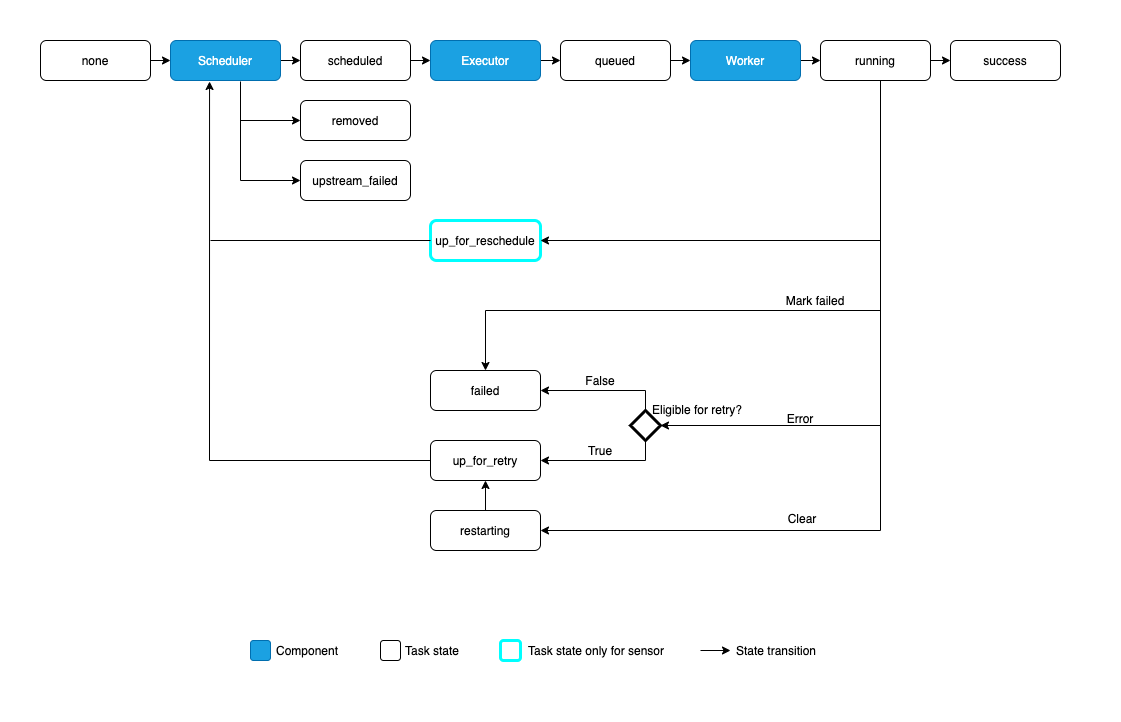
\includegraphics[width=0.8\textwidth]{img/task_lifecycle_diagram.png}
    \caption{Diagramma di tutti i possibili stati di una task}
    \label{fig:task_lifecycle}
\end{figure}

Come si può vedere in figura \ref{fig:task_lifecycle}, l'obiettivo ideale è che una task attraversi lo stato da none a success, passando per scheduled, queued e running. Per impostazione predefinita, una task viene eseguita solo se tutte le sue upstream (le task che la precedono nel flusso logico) sono completate con successo, ma Airflow offre anche strumenti avanzati di controllo del flusso (branching, trigger rules, ecc.).


\subsection{Architettura}
\label{sec:architettura}
L'architettura di Airflow è formata da diversi componenti. Un'installazione minima di Apache Airflow è formata in questo modo: 

\begin{itemize}
    \item \textbf{Scheduler}: Il cuore del sistema, si occupa di pianificare l'esecuzione dei workflow (DAG) secondo la programmazione definita, individuando i task che devono essere eseguiti e inviandoli all'esecutore (executor). L'executor, che è una proprietà configurabile dello scheduler, gestisce l'esecuzione dei task e può lavorare in modalità locale o distribuita, a seconda delle esigenze e delle risorse disponibili.
    \item \textbf{Webserver}: Fornisce un'interfaccia web intuitiva che permette di visualizzare, monitorare e gestire i DAG e i task, analizzare i log, forzare l'esecuzione manuale dei workflow e diagnosticare eventuali problemi.
    \item \textbf{Cartella /dags}: Una directory locale (o su storage condiviso) in cui risiedono i file Python che definiscono i DAG. Lo scheduler esegue periodicamente la scansione di questa cartella per individuare nuovi workflow o aggiornamenti ai workflow esistenti.
    \item \textbf{Meta Database}: Un database relazionale (tipicamente PostgreSQL o MySQL) utilizzato da tutti i componenti di Airflow per tracciare lo stato delle esecuzioni dei DAG e dei task, memorizzare configurazioni, cronologia delle esecuzioni, log degli errori e altri metadati fondamentali.
\end{itemize}

\begin{figure}[h]
    \centering
    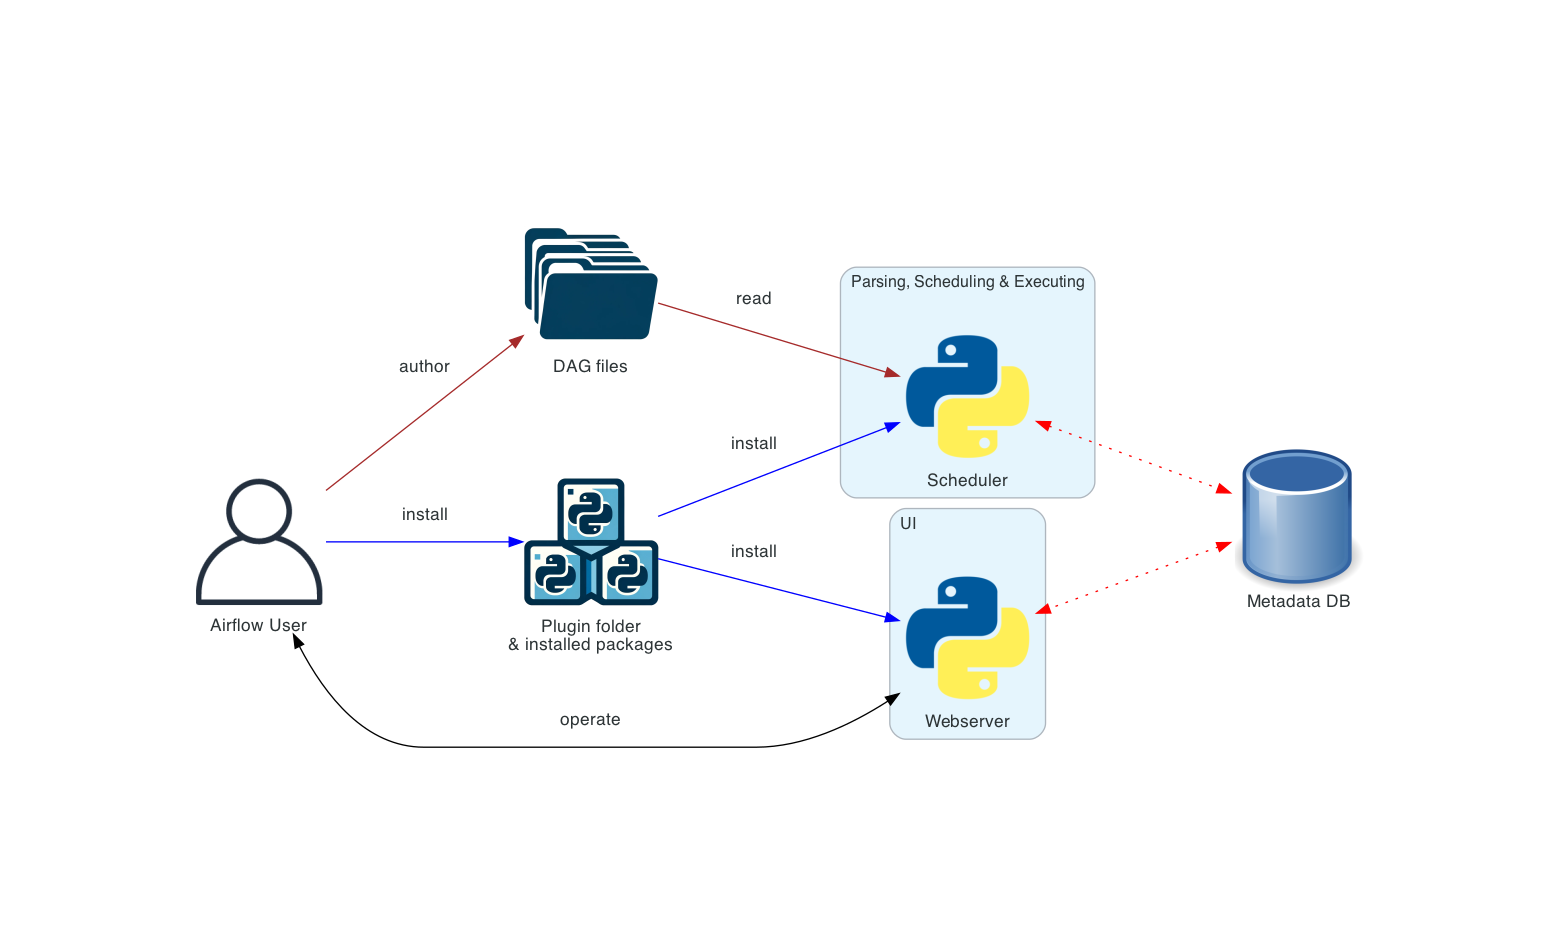
\includegraphics[width=0.8\textwidth]{img/diagram_basic_airflow_architecture.png}
    \caption{Fig 2.3 Diagramma del deployment minimo di Airflow}
    \label{fig:airflow_minimal_deployment}
\end{figure}

In figura ~\ref{fig:airflow_minimal_deployment} viene mostrata la configurazione più semplice di Airflow, in cui tutti i componenti principali (scheduler, webserver e database) vengono eseguiti sulla stessa macchina. In questo scenario si utilizza solitamente il LocalExecutor: scheduler e worker condividono lo stesso processo Python e i file dei DAG vengono letti direttamente dal filesystem locale. Anche l’interfaccia web (webserver) viene eseguita sulla stessa macchina. È importante far notare la differenza tra executor e worker: 
L’executor in Airflow determina la modalità e la logica con cui i task vengono messi in esecuzione, gestendo l’assegnazione dei task ai worker.
Il worker è invece il processo che riceve i task dall’executor e li esegue.

\subsection{Perché utilizzare Airflow?}
\label{sec:percheairflow}
Apache Airflow offre numerosi vantaggi nella gestione dei workflow. In primo luogo, la flessibilità della piattaforma consente di definire pipeline complesse come codice Python, integrandosi con praticamente qualsiasi tecnologia. Inoltre, l’automazione tramite la schedulazione integrata permette di eseguire i workflow a intervalli prestabiliti, e la gestione delle dipendenze garantisce che i task vengano eseguiti nell’ordine corretto secondo le relazioni definite. Airflow è altamente scalabile, potendo operare da un singolo processo locale fino a cluster distribuiti capaci di gestire carichi di lavoro ingenti. Offre anche un’ottima osservabilità: tramite un’interfaccia web si possono visualizzare chiaramente lo stato dei DAG, i log dei task e altri indicatori, facilitando il monitoraggio e il troubleshooting dei processi. Infine, sono previsti meccanismi di retry automatico e robusta gestione degli errori, così che eventuali fallimenti vengano intercettati e i task possono essere ritentati automaticamente per garantire la continuità delle pipeline.

\section{Monitoraggio e metriche}
\label{sec:monitoraggioemetriche}

Monitorare significa raccogliere, analizzare e visualizzare metriche e log per osservare il comportamento di un sistema nel tempo. Nell’ambito dell’informatica e dell’ingegneria del software, il monitoring si concentra principalmente sul tracciamento di metriche predefinite e indicatori chiave di performance (KPI) con l’obiettivo di rilevare deviazioni dal comportamento atteso.
Tipicamente vengono utilizzati strumenti di monitoring per raccogliere dati come utilizzo di CPU, memoria, tempo di risposta e tassi di errore. Questi dati vengono analizzati in tempo reale e, al superamento di determinate soglie, il sistema può inviare degli alert per consentire una risposta tempestiva a possibili problemi.

Nel mio progetto, il monitoring della pipeline dati è stato realizzato tramite l’integrazione di strumenti open source come StatsD, Prometheus e Grafana. Airflow esporta automaticamente metriche relative allo stato delle task, alle risorse utilizzate (CPU/RAM) e alla durata delle esecuzioni, che vengono poi raccolte e visualizzate in dashboard interattive. Questo consente di identificare rapidamente task fallite o anomalie di performance e intervenire in modo reattivo, garantendo affidabilità ed efficienza nella gestione dei workflow automatizzati.

\begin{figure}[h]
    \centering
    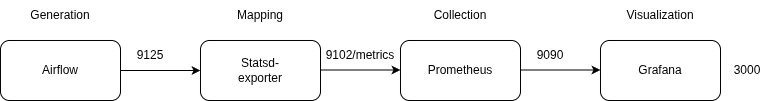
\includegraphics[width=0.8\textwidth]{img/monitoraggioschema.png}
    \caption{Schema logico dei servizi di estrazione metriche e monitoraggio}
    \label{fig:monitoring_schema}
\end{figure}

\subsection{StatsD e StatsD Exporter}
\label{sec:statsd}

\textbf{StatsD} è un \textit{network daemon} sviluppato da Etsy, progettato per raccogliere metriche inviate dalle applicazioni tramite protocolli leggeri come UDP o TCP. Ogni metrica è rappresentata dalla sintassi:

\begin{verbatim}
<nome_metrica>:<valore>|<tipo>
\end{verbatim}

dove il nome, espresso in notazione a punti (es. \texttt{dag.task.duration}), identifica la metrica, il valore è numerico e il tipo può indicare un contatore (\texttt{c}), un gauge (\texttt{g}), un timer (\texttt{ms}), ecc. Airflow utilizza questo formato per esportare automaticamente informazioni come l’avvio e il completamento delle task, la durata delle esecuzioni e l’uso delle risorse, inviandole in modo asincrono e a basso overhead.

Poiché il formato StatsD non è compatibile con Prometheus, entra in gioco lo \textbf{StatsD Exporter}, un servizio che traduce le metriche ricevute in serie temporali etichettate secondo lo standard Prometheus. La conversione è definita tramite un file di mapping in YAML, che permette di trasformare un nome di metrica come:

\begin{verbatim}
task.cpu_usage.vital_signs.process_dump:30|g
\end{verbatim}

nella forma Prometheus:

\begin{verbatim}
cpu_usage{dag="vital_signs", task="process_dump"} 30
\end{verbatim}

In questo modo le metriche diventano interrogabili con PromQL e possono essere visualizzate in Grafana. Dal punto di vista infrastrutturale, StatsD Exporter è stato configurato come servizio dedicato in \texttt{docker-compose.yml}, in ascolto sulla porta \texttt{9125} per ricevere i pacchetti StatsD da Airflow e sulla porta \texttt{9102} per esporre le metriche convertite a Prometheus.

\subsection{Prometheus}
\label{sec:prometheus}
Prometheus è una piattaforma open source progettata per il monitoraggio e l’alerting. È nata in SoundCloud e oggi fa parte della Cloud Native Computing Foundation.
Il suo funzionamento si basa su un approccio pull: invece di ricevere metriche dagli applicativi, Prometheus interroga periodicamente gli endpoint degli strumenti monitorati (ad esempio ogni 5 o 10 secondi) e raccoglie le metriche esposte in un formato testuale standard.
Queste metriche vengono archiviate come serie temporali, cioè insiemi di valori numerici associati a un timestamp e a un insieme di etichette (labels) che ne descrivono il contesto, ad esempio il nome del task o l’identificativo del DAG in Airflow.

Un aspetto centrale di Prometheus è la distinzione tra i tipi di metrica che le applicazioni possono esportare:

\begin{itemize}
    \item \textbf{Counter}: rappresenta un contatore che cresce monotonamente e può solo aumentare (o essere azzerato al riavvio). È usato ad esempio per il numero di richieste servite, task completate o errori riscontrati.
    \item \textbf{Gauge}: è un valore numerico che può sia aumentare che diminuire. Viene utilizzato per misurazioni istantanee come l’utilizzo della memoria, la temperatura, o il numero di processi attivi in un certo momento.
    \item \textbf{Histogram}: registra osservazioni (come la durata delle richieste o la dimensione delle risposte) suddividendole in bucket configurabili, e produce tre serie temporali: il conteggio cumulativo per bucket, la somma totale e il numero complessivo di osservazioni. È utile per calcolare quantili.
    \item \textbf{Summary}: simile all’histogram, campiona osservazioni e fornisce conteggio e somma, ma calcola direttamente quantili configurabili su una finestra temporale mobile. È adatto per ottenere metriche come la latenza mediana o il 95° percentile delle durate.
\end{itemize}

Prometheus offre diversi vantaggi:
\begin{itemize}
    \item conserva le metriche in un database ottimizzato per le serie temporali, permettendo query efficienti;
    \item utilizza un linguaggio dedicato, PromQL, che consente di analizzare e trasformare i dati (calcolare medie, percentili, confrontare valori tra task o host diversi);
    \item può generare regole di alerting, ad esempio inviando notifiche quando una metrica supera una certa soglia o quando un servizio non risponde più;
    \item si integra facilmente con strumenti di visualizzazione come Grafana, che permette di trasformare i dati raccolti in dashboard interattive.
\end{itemize}

\subsection{Grafana}
\label{sec:grafana}

Grafana è un’applicazione web open-source per analisi e visualizzazione di metriche, log e tracce da molteplici sorgenti dati. Consente di costruire dashboard interattive e condivisibili tramite un sistema di datasource (es. Prometheus, InfluxDB, Elasticsearch, SQL).
Serve a monitorare sistemi e applicazioni trasformando i dati (tipicamente serie temporali) in grafici, tabelle, gauge e heatmap; permette inoltre alerting, esplorazione ad-hoc e condivisione di dashboard.


Il funzionamento di Grafana si articola in alcuni passaggi fondamentali:

\begin{itemize}
    \item configurazione di una sorgente dati (ad esempio Prometheus);
    \item creazione di una dashboard, suddivisa in pannelli;
    \item ogni pannello contiene una o più query verso la sorgente dati e una relativa visualizzazione (grafico, tabella, gauge, ecc.);
    \item possibilità di utilizzare variabili di dashboard per filtrare i dati dinamicamente (ad esempio per DAG, task o host specifici);
    \item personalizzazione dei pannelli con legende, soglie e formattazioni per facilitare l’interpretazione.
\end{itemize}
Grafana ha un’integrazione nativa con Prometheus: una volta aggiunto come data source, Grafana può eseguire query direttamente tramite PromQL e trasformare i risultati in visualizzazioni interattive. Questo legame è uno dei motivi principali per cui Prometheus e Grafana vengono spesso adottati insieme: Prometheus si occupa della raccolta e conservazione delle metriche, mentre Grafana ne gestisce la presentazione e l’esplorazione.
Il linguaggio di interrogazione di Prometheus è PromQL (Prometheus Query Language), appositamente concepito per l’analisi delle serie temporali. Permette di estrarre valori istantanei (instant vector) e intervalli temporali (range vector), ed include funzioni come rate(), nonché operatori aritmetici e aggregati, utili per calcolare medie, percentili e confronti tra metriche. In Grafana, le query scritte in PromQL alimentano i pannelli, consentendo di trasformare dati grezzi in visualizzazioni significative.


Un esempio di query PromQL potrebbe essere:
\begin{verbatim}
    rate(node_disk_written_bytes_total{job="integrations/macos-node", device!=""}[5m])
\end{verbatim}

Questa query calcola la velocità di scrittura su disco in byte al secondo negli ultimi 5 minuti, filtrando per il job specifico e ignorando i dispositivi vuoti. Il risultato può essere visualizzato in un grafico a linee o in un gauge, a seconda delle preferenze dell'utente.
La funzione rate() in PromQL calcola la velocità media di incremento al secondo di una metrica di tipo counter, valutata su un intervallo temporale specificato (es. ultimi 5 minuti).

\begin{figure}[h]
    \centering
    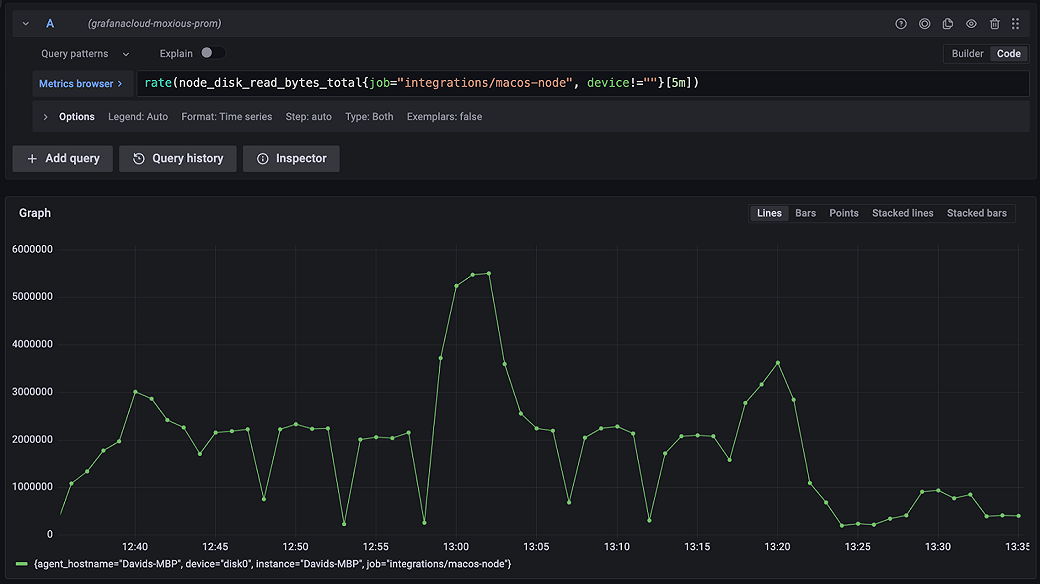
\includegraphics[width=0.8\textwidth]{img/rate-function.png}
    \caption{Esempio di visualizzazione di una query PromQL in Grafana che mostra la velocità di scrittura su disco}
    \label{fig:rate_function_example}
\end{figure}


